\section{ADC Sampling and Burst Timing}
\label{sec:ctrl-architecture}

The Arduino STM32 framework was used with direct peripheral configuration. Center-aligned TIM1 generates the carrier commands at PA8/PA9: \SI{1}{\mega\hertz} with a nominal \SI{40}{\nano\second} dead interval at both transitions. TIM3 schedules burst enable at PA10. Before non-static enable transitions, bounded polling attempts to align the edge with a TIM1 update; timeout can occur without an observed update. Static \SI{100}{\percent} command holds PA10 high without repeated gaps. A low enable inhibits further switching but does not discharge the power-circuit capacitors.

ADC1 sequentially samples primary voltage at PA0, secondary-bulk voltage at PA1, and half-bridge current at PA2 into a circular DMA buffer. The scan is free-running without synchronization to the carrier, and DMA acquisition continues while the foreground loop runs. Each control pass converts and filters the latest samples, evaluates state and faults, and sends a duty request to the enable scheduler. A hardware UART carries commands and status.

\begin{figure}[htbp]
\centering
\begingroup
\definecolor{ctrlnavy}{HTML}{153448}
\definecolor{ctrlteal}{HTML}{007C83}
\definecolor{ctrlred}{HTML}{990000}
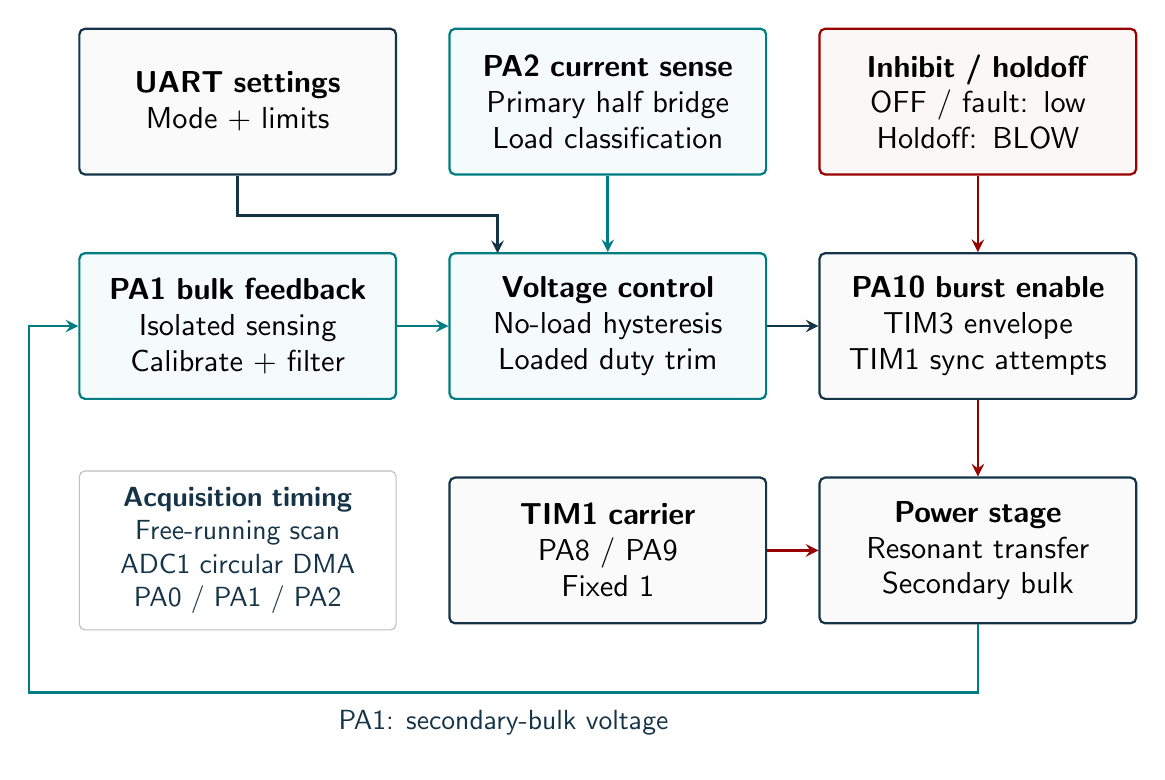
\begin{tikzpicture}[
font=\sffamily\fontsize{11}{13}\selectfont,
every node/.style={align=center,inner sep=6pt,
    execute at begin node={\hyphenpenalty=10000\exhyphenpenalty=10000}},
block/.style={draw=ctrlnavy,fill=black!2,rounded corners=2pt,
    line width=0.8pt,text width=3.6cm,minimum height=1.85cm},
ctrl/.style={block,draw=ctrlteal,fill=ctrlteal!4},
protect/.style={block,draw=ctrlred,fill=ctrlred!3},
flow/.style={->,>=stealth,draw=ctrlnavy,line width=1.0pt},
senseflow/.style={flow,draw=ctrlteal},
command/.style={flow,draw=ctrlred},
annotation/.style={font=\sffamily\fontsize{10}{12}\selectfont,text=ctrlnavy}]
\node[ctrl] (sense) at (0,0)
    {\textbf{PA1 bulk feedback}\\Isolated sensing\\Calibrate + filter};
\node[ctrl] (control) at (4.7,0)
    {\textbf{Voltage control}\\No-load hysteresis\\Loaded duty trim};
\node[block] (en) at (9.4,0)
    {\textbf{PA10 burst enable}\\TIM3 envelope\\TIM1 sync attempts};
\node[block] (plant) at (9.4,-2.85)
    {\textbf{Power stage}\\Resonant transfer\\Secondary bulk};
\node[block] (uart) at (0,2.85)
    {\textbf{UART settings}\\Mode + limits};
\node[ctrl] (load) at (4.7,2.85)
    {\textbf{PA2 current sense}\\Primary half bridge\\Load classification};
\node[protect] (fault) at (9.4,2.85)
    {\textbf{Inhibit / holdoff}\\OFF / fault: low\\Holdoff: BLOW};
\node[block] (carrier) at (4.7,-2.85)
    {\textbf{TIM1 carrier}\\PA8 / PA9\\Fixed \SI{1}{\mega\hertz}};
\node[annotation,draw=black!25,fill=white,rounded corners=2pt,
    text width=3.6cm,minimum height=1.85cm] at (0,-2.85)
    {\textbf{Acquisition timing}\\Free-running scan\\ADC1 circular DMA\\PA0 / PA1 / PA2};
\draw[senseflow] (sense) -- (control);
\draw[flow] (control) -- (en);
\draw[command] (en) -- (plant);
\draw[senseflow] (load) -- (control);
\draw[flow] (uart.south) -- (0,1.4) -- (3.3,1.4) -- (3.3,0.925);
\draw[command] (fault) -- (en);
\draw[command] (carrier) -- (plant);
\draw[senseflow] (plant.south) -- (9.4,-4.65) --
    node[annotation,below,fill=white] {PA1: secondary-bulk voltage}
    (-2.65,-4.65) -- (-2.65,0) -- (sense.west);
\end{tikzpicture}
\endgroup
\caption{Baseline control loop and timing. PA1 provides secondary-bulk voltage feedback; PA2 provides primary-current feedback for load detection. PA10 enables bursts and PA8/PA9 generate the fixed carrier. OFF/fault drives PA10 low; soft holdoff requests \texttt{BLOW}, which is zero by default.}
\label{fig:ctrl-software-architecture}
\end{figure}

\begin{table}[htbp]
\centering
\caption{Timers, ADC, and UART used by the baseline firmware.}
\label{tab:fw-identity-timing-record}
\begin{tabularx}{\textwidth}{@{}p{0.22\textwidth}p{0.27\textwidth}X@{}}
\toprule
Peripheral & MCU pins & Function\\
\midrule
TIM1 & PA8 and PA9 & Fixed carrier and attempts to align enable edges\\
TIM3/GPIO & PA10 & Enable-period scheduling and power-stage inhibition\\
ADC1/DMA1 & PA0, PA1, PA2 & Continuous sampling of the three inputs\\
Hardware UART & PC5 RX, PC4 TX & \SI{115200}{baud} commands, status, and export\\
\bottomrule
\end{tabularx}
\end{table}

Background command parsing is bounded per pass, and settings writes are inhibited while output is enabled to limit control delays. Software counters record observed execution intervals; external timing captures are needed to measure their jitter.
